\chapter{Analysis techniques}

\intro{This chapter introduces the necessary toolset to perform the analyses within this thesis. It is organized to follow the common steps of the analyses. First, the generation of simulated events is introduced. Then, details of the top quark reconstruction, the employed multivariate analysis technique, and the template fit is given which are used to estimate the amount of single top quark events within the recorded data. Lastly, the partonic and fiducial objects are defined to which the observed data is unfolded to for comparison with theoretical predictions.}

%##############################################
\section{Event generation}
%##############################################

To compare reconstructed data with theoretical predictions, samples of simulated events are generated from theory and passed through a simulation of the \gls{cms} detector and emulation of its readout. The standard so-called ``FullSimulation'' package~\cite{1742-6596-396-2-022003,1742-6596-664-7-072022} is based on the Geant4 toolkit~\cite{Agostinelli2003250} which provides a detailed simulation of particle trajectories and interactions with the detector material. A fast alternative, the so-called ``FastSimulation'' package, exists within \gls{cms} as well~\cite{fsimRahmat} but has not been used for simulating the detector response in the analyses within this thesis.

The event generation starts with the \glshere{me} of a hard scattering process of interest. \glshere{mc} methods are employed to sample the corresponding cross section integral. The advantage of \gls{mc}-based methods is that the variance of their result decreases as $1/n$ independently of the integral's dimensionality leading to an efficient convergence compared to quadrature-based methods~(e.g. Simpson's rule, Newton-Cotes). A common method to integrate cross sections is given by the \gls{vegas} algorithm~\cite{OHL199913}. It is based on importance sampling where the integral is sampled not uniformly but along an adaptive importance function instead. The resulting sample of events reflects the probability distribution of a process over its phase space. Typically a reweighting is performed in addition such that all events contribute the same probability (e.i. they carry the same absolute weight). 

After obtaining events from the hard interaction, a \glshere{ps} program simulates the hadronization of final state partons. In addition, the radiation of gluons or quarks from initial or final state partons is accounted for as well as contributions from soft secondary interactions, the so-called underlying event, and potential color reconnection effects. A sketch of various parts within an exemplary pp collision event after hadronization is shown in Fig.~\ref{fig:technique-mcevent}. The \gls{ps} simulation is based on Altarelli-Parisi splitting functions~\cite{Altarelli:1977zs} which allow to calculate the probability of soft parton emissions, e.g. $\mathrm{q}\to \mathrm{gq}$. It is convenient to calculate the ``surviving'' probability, the so-called Sudakov factor, that a parton does not branch further below a certain energy scale. During the \gls{ps} simulation a complication arises from potential double counting of soft parton emissions since the simulation of the hard interaction may lead to a soft emission as well which is however already accounted for by the \gls{ps}. These are avoided by applying a dedicated \gls{me}-to-\gls{ps} matching scheme, depending on the \gls{ps} program, which yields a criterion to assign additional emissions to either the simulation of the hard interaction or the \gls{ps} exclusively depending on the event kinematics. More information on parton shower simulation and matching can be found in Refs.~\cite{Hoche:2014rga,Alwall:2007fs}.


\myfigure{\label{fig:technique-mcevent} A sketch of a generated event from the simulation of the hard interaction and subsequent hadronization through a parton shower. The figure is taken in parts from Ref.~\cite{Hoche:2014rga}.}{
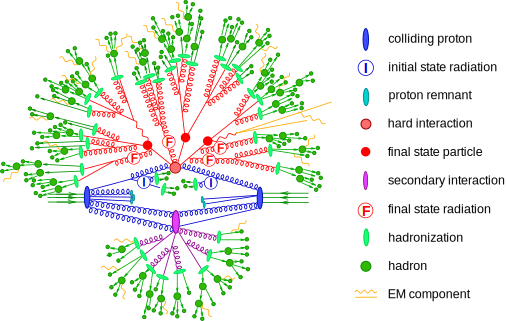
\includegraphics[scale=0.75]{figures/technique/shower.pdf}
}

A brief overview of the programs used for generation and subsequent hadronization of $t$-channel single top quark production is given in the following.

\begin{description}
\item[MadGraph5\_aMC{@}NLO] The \MGAMC program~\cite{Alwall:2014hca} is a merge of the \gls{lo} \MG generator~\cite{Alwall:2011uj} and \AMC into a common framework. It supports the generation of \gls{lo} or \gls{nlo} samples which can be matched to parton showers using the MLM~\cite{Mangano:2006rw} or MC{@}NLO~\cite{Frixione:2002ik} schemes respectively. The latter method produces a certain fraction of events with negative weights (depending on the process) which stem from a subtraction of additional emissions from the \gls{nlo} matrix element to prevent double-counting. 
Multiple samples of events with additional final state partons at matrix element level can also be merged into a combined sample. Here, the overlap with the \gls{ps} is removed through the FxFx merging scheme~\cite{Frederix:2012ps}.

\item[Powheg] The \POWHEG box (versions~1,2)~\cite{Alioli:2010xd} is a program that contains predefined implementations of various processes such as $t$-channel single top quark production~\cite{Alioli:2009je} at \gls{nlo}. It utilizes the so-called \POWHEG method~\cite{Frixione:2007vw} for matching in which the hardest radiation generated from the \gls{me} has priority over subsequent \gls{ps} emissions. This removes the overlap with the \gls{ps} without the generation of negatively weighted events.

\item[CompHEP] The \COMPHEP program (version~4.5)~\cite{Boos:2004kh} can perform calculations of cross sections from Lagrangians at \gls{lo}. In addition, generation of events is also possible such as single top quark production~\cite{Boos:2006af}. Here, an approximation is used by combining events from the $2\to2$ and $2\to3$ processes which reproduces effectively \gls{nlo} corrections.

\item[Pythia] The \PYTHIA program (versions~6,8)~\cite{Sjostrand:2006za,Sjostrand:2014zea} can generate events of various processes at \gls{lo}. It is however famous for its \gls{ps} simulation which can be interfaced with other \gls{lo} and \gls{nlo} event generators to perform subsequent parton showering, hadronization, and the simulation of the underlying event. For hadronization, a phenomenological model is utilized in which one-dimensional strings\footnote{The string model is motivated by the fact that the spatial form of a dipole color field does not extend radially like an \gls{em} field but is instead squeezed to a tube-like form.} connected to partons reflect the color field leading to the creation of additional partons through string branching and finally to the formation of color-neutral singlets.

\item[Herwig++] The \HERWIG program (version~7)~\cite{Bellm:2015jjp} is an \gls{nlo} event generator which is also capable of simulating the showering of partons similar to \PYTHIA. Its hadronization algorithm utilizes a model in which color-connected quarks are spatially kept together in clusters~\cite{Webber:1983if} which is motivated by the ``preconfinement'' of color~\cite{Amati:1979fg}. If the mass of a cluster is sufficiently high it can decay into lighter clusters with a certain probability. In its final step, a cluster decays then into a pair of hadrons.
\end{description}




%##############################################
\section{Top quark reconstruction}
%##############################################

After the reconstruction and selection of analysis objects, a top quark candidate is reconstructed in the presented analyses. Assuming that the top quark decayed leptonically as $\mathrm{t}\to\mathrm{b}\mathrm{W}\to\mathrm{b}\ell\nu$ its energy and momentum is reconstructed by summing the measured 4-momenta of a selected lepton (muon or electron), b-tagged jet, and neutrino candidate. The neutrino candidate itself is reconstructed from the missing transverse energy and the lepton momentum by requiring a W~boson mass constraint of $m_\mathrm{W}=80.4~\GeV$~\cite{Olive:2016xmw} on their invariant mass as

\begin{align}
m_\mathrm{W}^2=\colvec{2}{E_\mathrm{W}}{\vec{p}_\mathrm{W}}^{2}&\overset{!}{=}\left[\colvec{2}{E_{\ell}}{\vec{p}_{\ell}}+\colvec{2}{E_{\nu}}{\vec{p}_{\nu}}\right]^{2}\nonumber\\
&=\underbrace{m_{\ell}^2+m_{\nu}^2}_{\approx 0}+\,2\cdot E_{\ell}\,E_{\nu}-\,2\cdot\colvec{3}{p_{\ell,x}}{p_{\ell,y}}{p_{\ell,z}}\cdot\colvec{3}{p_{\nu,\mathrm{T}}\cdot\cos\phi_{\nu}}{p_{\nu,\mathrm{T}}\cdot\sin\phi_{\nu}}{p_{\nu,z}}. \label{eq:technique-neutrino-pz-eq}
\end{align}

When taking $p_{\nu,\mathrm{T}}$ and $\phi_{\nu}$ from the missing transverse momentum vector $\pvmiss$, this allows to solve for the unknown $p_{\nu,z}$-component of the neutrino candidate momentum. After rearranging, one obtains from Eq.~\ref{eq:technique-neutrino-pz-eq} the quadratic equation

\begin{equation}
0=p_{\nu,z}^2-\frac{2\,\xi\,p_{\ell,z}}{E_{\ell}^{2}-p_{\ell,z}^2}\cdot p_{\nu,z}-\frac{\xi^{2}-E_{\ell}^{2}\,p_{\nu,\mathrm{T}}^2}{E_{\ell}^{2}-p_{\ell,z}^2},\end{equation}

with

\begin{equation}
\xi=\frac{m_\mathrm{W}^2}{2}+p_{\nu,\mathrm{T}}\,p_{\ell,\mathrm{T}}\cdot\cos\big(\phi_\ell-\phi_\nu\big)
\end{equation}

which possesses the solutions

\begin{align}
p_{\nu,z}^{1,2}=\frac{1}{E_{\ell}^{2}-p_{\ell,z}^{2}}\left[\xi\cdot p_{\ell,z}\pm E_{\ell} \sqrt{\xi^2-p_{\nu,\mathrm{T}}^2\big(E_{\ell}^2-p_{\ell,z}^2\big)}~\right]. \label{eq:technique-neutrino-pz}
\end{align}

A detailed derivation and discussion of this result can be found in Ref.~\cite{Chwalek:1416031}. In simulated $t$-channel single-top-quark events this procedure leads to two real solutions for the neutrino $p_{\nu,z}$-component in about 65\% of all events that passed the selection. From the two solutions the one with the smallest absolute $|p_{\nu,z}|$ is chosen which is found to be closest to the true neutrino $p_{z}$ in 63\% of events with real solutions. In the remaining 37\% of events, both real solutions are found to be close together \todo{how close} such that the mistake here by picking the smallest solution is acceptable. If the discriminant in Eq.~\ref{eq:technique-neutrino-pz} becomes negative the solutions are complex. This happens in about 35\% of events and occurs mostly due to the finite \met resolution whereas the negligence of the W~boson mass width and resolution of the lepton momentum are minor effects. The imaginary part of the solutions is removed by requiring that the discriminant vanishes

\begin{equation}
0\overset{!}{=}\xi^2-p_{\nu,\mathrm{T}}^2\big(E_{\ell}^2-p_{\ell,z}^2\big)~
\Rightarrow~ p_{\nu,z}=\frac{\xi\cdot p_{\ell,z}}{E_{\ell}^{2}-p_{\ell,z}^{2}}
\end{equation}

which is equal to setting the transverse W~boson mass $\mtw$ to the W~boson mass itself

\begin{align}
m_\mathrm{W}^2\overset{!}{=}\mtw^2&=(p_{\ell,\mathrm{T}}+p_{\nu,\mathrm{T}})^2-(p_{\ell,x}+p_{\nu,x})^{2}-(p_{\ell,y}+p_{\nu,y})^{2}\\
&=2\,p_{\ell,\mathrm{T}}^2\,p_{\nu,\mathrm{T}}^2\cdot\Big[1-\cos\big(\phi_\ell-\phi_\nu\big)\Big].
\end{align}

Then, the $p_{\nu,x}$ and $p_{\nu,x}$ components are varied and the transverse momentum which minimizes the distance $|\vec{p}_{\nu,\mathrm{T}}-\pvmiss|$ with respect to the measured missing momentum vector is taken as the result. 

\todo{show improvement of MET res in case of complex solutions}

\todo{top quark matching performance
(top pT/eta as function of b-tag in acceptance after selection, b-quark within dR, top within dR)}

%##############################################
\section{Boosted Decision Trees}
%##############################################

Typically, the $t$-channel single-top-quark signal region, defined by one isolated lepton, 2~jets (where one is b-tagged), and significant \met, is found to be still largely contaminated by events from background processes after the event selection. In measurements of the production cross section at 8~and 13~TeV, the ratios of the signal yield over the total background yield are about 13\% and 14\%  respectively~\cite{Khachatryan:2014iya,Sirunyan:2016cdg}\todo{update TOP-16-003 when accepted by PRL}. The majority of background events stem from \wjets and \ttbar production.

An observable to separate signal from background events is given by the pseudorapidity of the spectator jet, $\eta(\jprime)$, which 


 can be obtained from \glshere{mva} techniques such as \glsplhere{nn} or \glsplhere{bdt}. In this thesis, \glspl{bdt} have been employed to extract the amount of signal events.
\cite{Hocker:2007ht}

%##############################################
\section{Template-based fitting}
%##############################################

likelihood, barlow-beeston method

%##############################################
\section{Partonic and fiducial objects}
%##############################################

dressed leptons, jet clustering, b-tagging

%##############################################
\section{Unfolding}
%##############################################

problems, regularization scheme, correlations, subway plot, alternative FBU
